\documentclass[twoside]{article}
\usepackage{amsmath}
\usepackage{amssymb}
\usepackage{algorithm}  
\usepackage{algorithmicx}  
\usepackage{algpseudocode}  
\usepackage{amsmath}  

  
\renewcommand{\algorithmicrequire}{\textbf{Input:}}  
\renewcommand{\algorithmicensure}{\textbf{Output:}} 
\usepackage{epsfig} 
\usepackage{graphicx}
\usepackage{subfigure}

\setlength{\oddsidemargin}{0.25 in}
\setlength{\evensidemargin}{-0.25 in}
\setlength{\topmargin}{-0.6 in}
\setlength{\textwidth}{6.5 in}
\setlength{\textheight}{8.5 in}
\setlength{\headsep}{0.75 in}
\setlength{\parindent}{0 in}
\setlength{\parskip}{0.1 in}

\newcommand{\lecture}[3]{
   \pagestyle{myheadings} 
   \thispagestyle{plain}
   \newpage
   \setcounter{page}{1}
   \noindent
   \begin{center}
   \framebox{
      \vbox{\vspace{2mm}
    \hbox to 6.28in { {\bf 10-707: Deep Learning, Fall 2017 \hfill} }
       \vspace{6mm}
       \hbox to 6.28in { {\Large \hfill #1  \hfill} }
       \vspace{6mm}
       \hbox to 6.28in { {\it Lecturer: #2 \hfill Name: #3} }
      \vspace{2mm}}
   }
   \end{center}
   \markboth{#1}{#1}
   \vspace*{4mm}
}

\begin{document}

\lecture{Homework 1}{Russ Salakhutdinov }{Yuan Liu(yuanl4)} % Lecture name, Lecturer, Scribes
\section{Problem 1}
\subsection{Error vs model complexity}
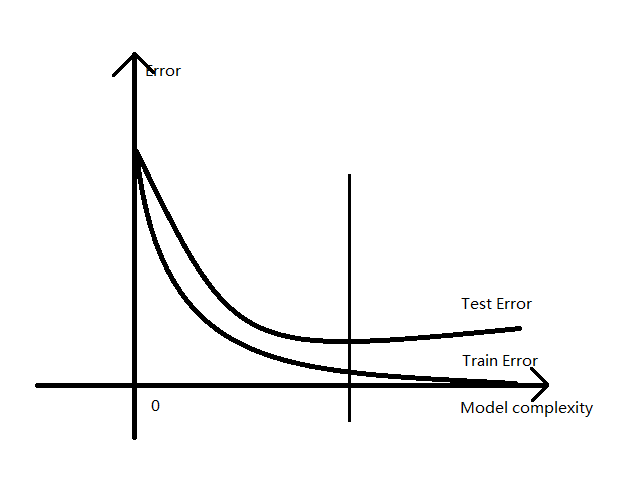
\includegraphics[width=0.5\linewidth]{images/1_1}

\subsection{Error vs size of training dataset}
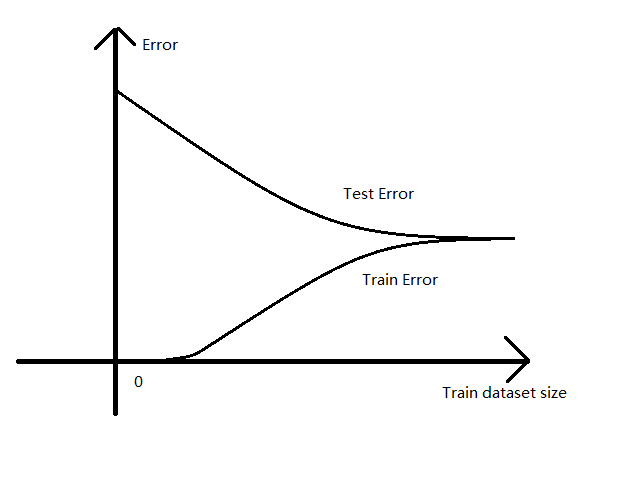
\includegraphics[width=0.5\linewidth]{images/1_2}

\subsection{Early stopping}
\paragraph{} Early stopping is a reasonable regularization metric. Machine learning algorithms train a model based on a finite set of training data with an iterative method. The goal of machine learning is to predict the unseen observations.  Up to a point, the iterative update methods improves the model's performance on unseen observations. Past that point, overfitting occurs.  Early stopping rules provide guidance as to how many iterations can be run before the learner begins to over-fit.

\section{Problem 2}
\begin{itemize}
\item K-nearest-neighbor regression:
\paragraph{} For knn, the estimator is given by:
$$\hat f(x^*)= \frac{1}{k}\sum_{i\in N_k(x^*)}y_i$$
$N_k(x^*)$ contains the indices of the k closest points of $x_1,\dots,x_N$ to $x^*$.
Then we can know:
\begin{eqnarray}
l_i(x^*; \mathcal{X})=
\begin{cases}
\frac{1}{k}, & i\in N_k(x^*)\cr
 0, & otherwise 
 \end{cases}
\end{eqnarray}

\item Linear regression:
For linear regression, the estimator is given by:
$$\hat f(x^*) = {x^*}^Tw$$
where $w = (X^TX)^{-1}X^Ty$, $y=(y_1, \dots, y_N)^T$ and $X=(x_1,\dots, x_N)^T$. Then we can get:
$$\hat f(x^*) = {x^*}^T(X^TX)^{-1}X^Ty$$
So $$l_i(x^*; \mathcal{X}) =  ({x^*}^T(X^TX)^{-1}X^T)_i$$
$l_i(x^*; \mathcal{X})$ equals to the $i_{th}$ component of ${x^*}^T(X^TX)^{-1}X^T$.

\end{itemize}


\section{Problem 3}
\begin{itemize}
\item Normalization: $p(x=1|\mu)+p(x=-1|\mu) = \frac{1+\mu}{2}+\frac{1-\mu}{2}=1$
\item Mean:  $E[x]=1*p(x=1|\mu) + (-1)*p(x=-1|\mu)=\mu$
\item Variance: $Var[x]=E[x^2]-(E[x])^2 = \frac{1+\mu}{2}+\frac{1-\mu}{2} - \mu^2 = 1-\mu^2$
\item Entropy: $Entropy = -\sum_{i\in \{-1, 1\}} p(x=i|\mu) \log p(x=i|\mu) = - \frac{1+\mu}{2}\log \frac{1+\mu}{2}- \frac{1-\mu}{2}\log \frac{1-\mu}{2}$
\end{itemize}

\section{Problem 4}
\paragraph{}Denote $l$ is the correct label of $x$, and $t$ is the label of $x$ given by the dataset.
So we can have the following formula:
$$p(l = 1 | t=1) = 1-\epsilon$$
$$p(l = 1 | t=0) = \epsilon$$
\begin{align*}
p(l=1 | x; w) &= p(t=1| x; w)p(l=1|t=1)+p(t=0| x; w)p(l=1|t=0)\\
&=y(x, w)(1-\epsilon) + (1-y(x, w))\epsilon 
\end{align*}
Then we can get:
$$l \sim Bernoulli\left(y(x, w)(1-\epsilon) + (1-y(x, w))\epsilon\right)$$
$$p(l |x, w) =\left[y(x, w)(1-\epsilon) + (1-y(x, w))\epsilon\right]^{l}[1-y(x, w)(1-\epsilon) - (1-y(x, w))\epsilon]^{1-l}$$
\begin{align*}
\text{cost function} &= - \log p(l |x, w)\\
&= - l \log(y(x, w)(1-\epsilon) + (1-y(x, w))\epsilon ) - (1-\l) log(1-y(x, w)(1-\epsilon) - (1-y(x, w))\epsilon )\\
&= -l * \log(y-2y\epsilon+\epsilon) - (1-l) * \log(1-y+2y\epsilon-\epsilon)
\end{align*}
Where $l$ is the label of training dataset, $y$ is the output of neural network.

\paragraph{} If $\epsilon=0$, then $$\text{cost function} = -l * \log y - (1-l) *log(1-y)$$ which is the standard negative log likelihood of binary classification.

\section{Problem 5}
First represent two networks in the following form:
\begin{itemize}
\item Sigmoid network: Input $x=(x_1, \dots, x_p)^T$, First Layer: $a^{sig} = W^{sig}_{1}x + b^{sig}_1$, Activation function: $h^{sig} = \sigma (a^{sig})$, Second Layer: $o^{sig} = W^{sig}_2 h^{sig} + b^{sig}_2$

\item Tanh network: Input $x=(x_1, \dots, x_p)^T$, First Layer: $a^{tanh} = W^{tanh}_{1}x + b^{tanh}_1$, Activation function: $h^{tanh} = tanh (a^{tanh})$, Second Layer: $o^{tanh} = W^{tanh}_2 h^{tanh} + b^{tanh}_2$
\end{itemize}

By observation we can have:
$$\sigma(2a) = \frac{tanh(a)+1}{2}$$
First, we can assume:
$$W_1^{sig} = 2W_1^{tanh},\ \ \ b_1^{sig}=2b_1^{tanh}$$
Then $$a^{sig} = W^{sig}_{1}x + b^{sig} = 2W_1^{tanh}x+2b_1^{tanh} = 2 a^{tanh}$$
$$h^{sig}=\sigma(2 a^{tanh}) = \frac{tanh(a^{tanh})+1}{2}=\frac{h^{tanh}+1}{2}$$

Second, we can assume:
$$W_2^{sig} = 2W_2^{tanh},\ \ \ b_2^{sig}=b_2^{tanh}-W_2^{tanh} \cdot \mathbf{1}$$
Where $\mathbf{1}$ is a vector and all its component is 1.Then $$o^{sig} =  W^{sig}_2 h^{sig} + b^{sig}_2=2W_2^{tanh}\frac{h^{tanh}+\mathbf{1}}{2} +b_2^{tanh}-W_2^{tanh} \cdot \mathbf{1}=o^{tanh} $$
As a result, we can have the following equation:
$$W_1^{sig} = 2W_1^{tanh},\ \ \ b_1^{sig}=2b_1^{tanh}$$
$$W_2^{sig} = 2W_2^{tanh},\ \ \ b_2^{sig}=b_2^{tanh}-W_2^{tanh} \cdot \mathbf{1}$$

\section{Problem 6}
\subsection{(a)}
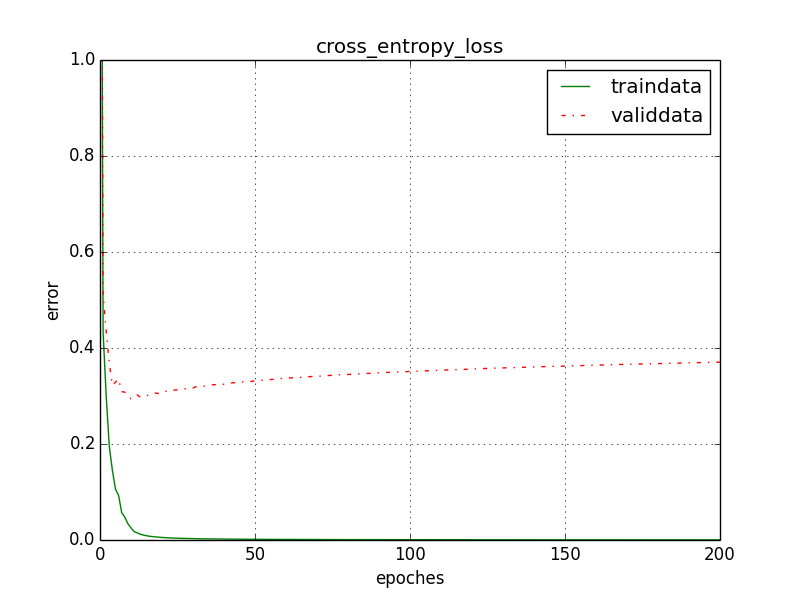
\includegraphics[width=0.5\linewidth]{images/problem_a}
\paragraph{} When the training is going on, the training error will keep decreasing. The validation error will first decrease, then up to a point, begins to increase. \\
The network's performance keeps becoming better and better on the training dataset. The network's performance on the validation dataset will first become better then becomes worse, because of over-fitting.


\subsection{(b)}
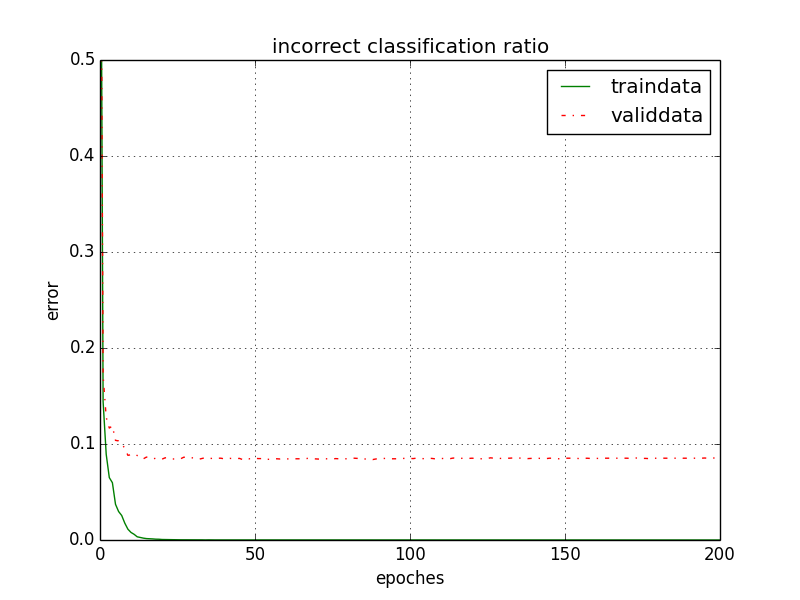
\includegraphics[width=0.5\linewidth]{images/problem_b}
\paragraph{} The over-fitting is difficult to be observed by the classification error.


\subsection{(c)}
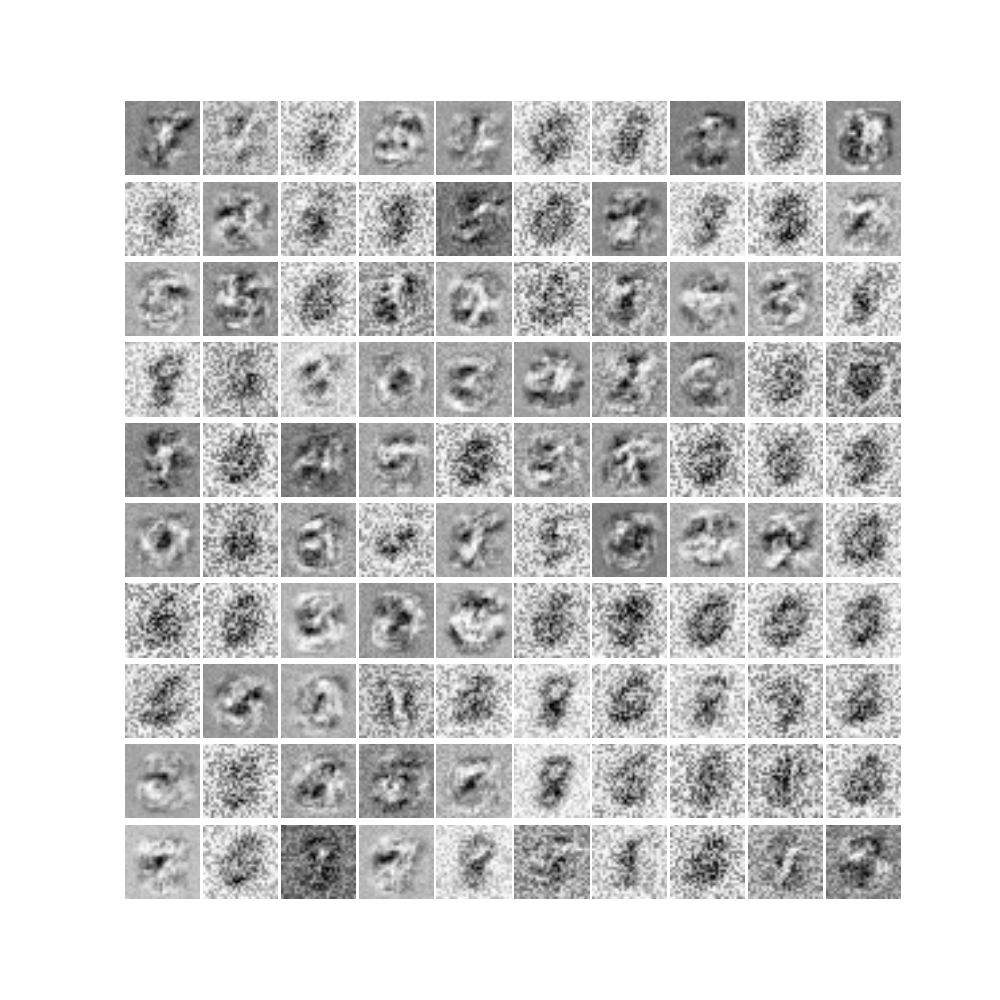
\includegraphics[width=0.5\linewidth]{images/problem_c}
\paragraph{} For example the sub-image on row 10 column 9 looks like number 1, the sub-image on row 4 column 5 looks like number 3, the sub-image on row 9 column 7 looks like number 8. I think this model can learn some structured  features.

\subsection{(d)}
\begin{figure}[h]
\centering
\subfigure[Problem d: different learning rate]{
\begin{minipage}[b]{0.4\textwidth}
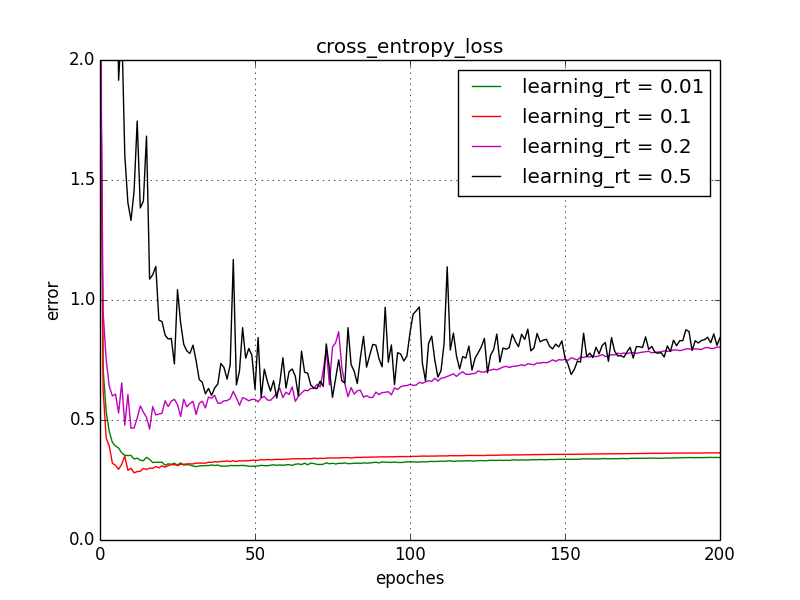
\includegraphics[width=1\textwidth]{images/problem_d_learning_rt_cross_entropy} \\
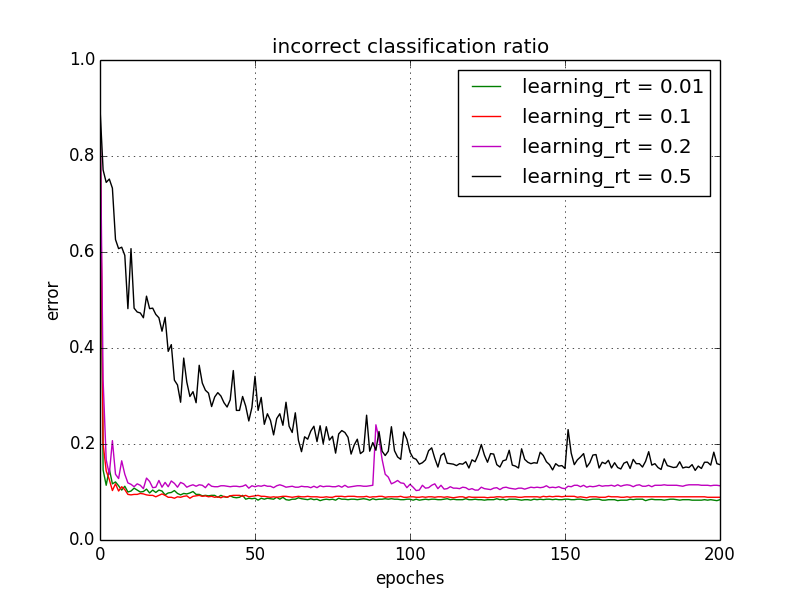
\includegraphics[width=1\textwidth]{images/problem_d_learning_rt_IC}
\end{minipage}
}
\subfigure[Problem d: different momentum]{
\begin{minipage}[b]{0.4\textwidth}
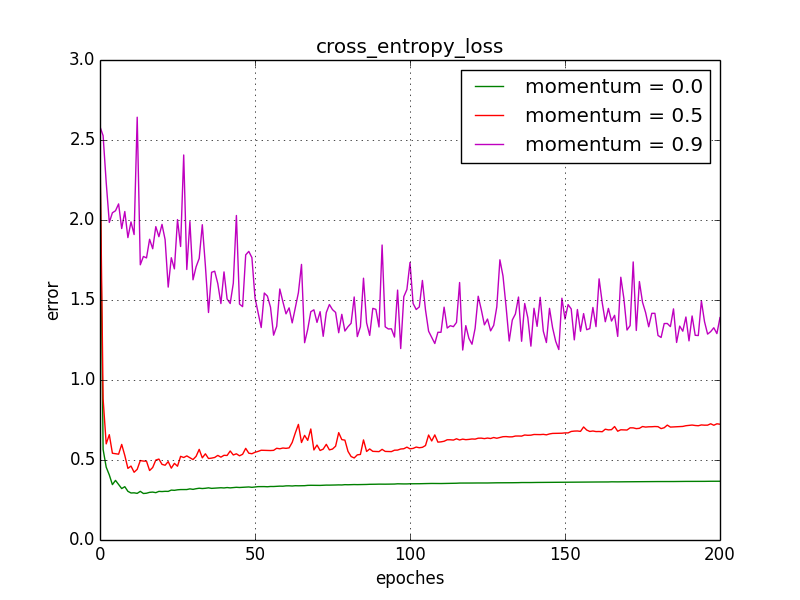
\includegraphics[width=1\textwidth]{images/problem_d_momentum_cross_entropy} \\
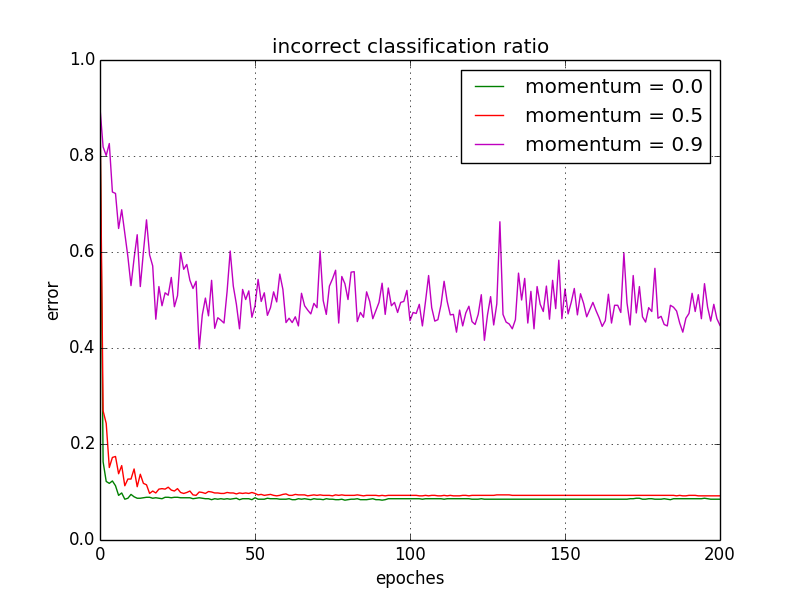
\includegraphics[width=1\textwidth]{images/problem_d_momentum_IC}
\end{minipage}

}
\end{figure}

\paragraph{} For this case, decreasing the learning rate will improves the model's performance and the momentum makes the model's performance worse. So I will choose learning rate equals 0.01 and momentum equals 0

\subsection{(e)}
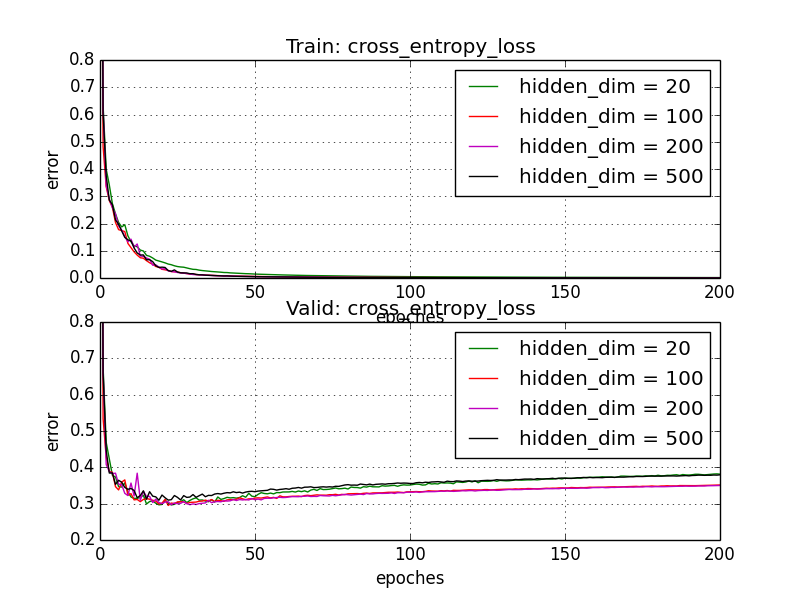
\includegraphics[width=0.5\linewidth]{images/problem_e}
\paragraph{}
$Hidden\ dimension = 100\ or\ 200$ is most suitable for this task. When the number of hidden units is too little or too much, the performance of network will become worse.

\subsection{(f)}

\begin{figure}[h]
\centering
\subfigure[Problem f: different L2 coefficients]{
\begin{minipage}[b]{0.4\textwidth}
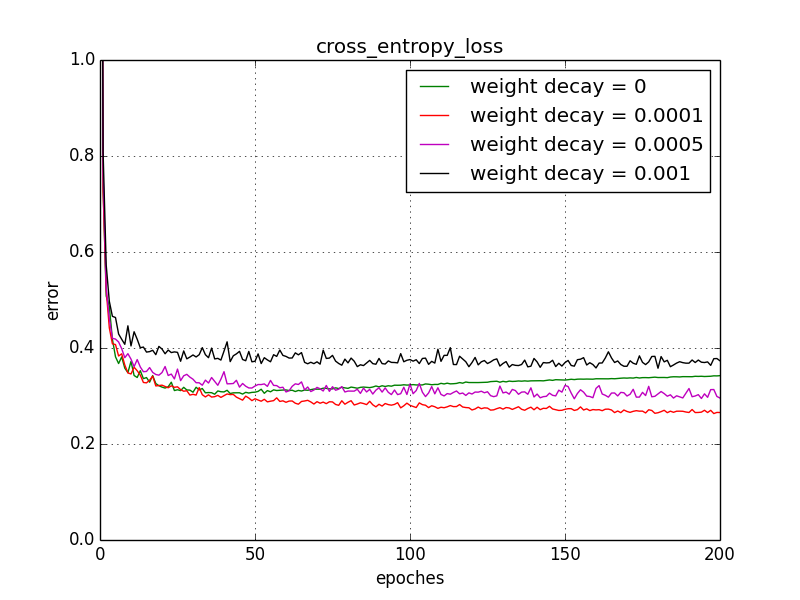
\includegraphics[width=1\textwidth]{images/problem_f_find_l2} 
\end{minipage}
}
\subfigure[Problem f: visualization]{
\begin{minipage}[b]{0.4\textwidth}
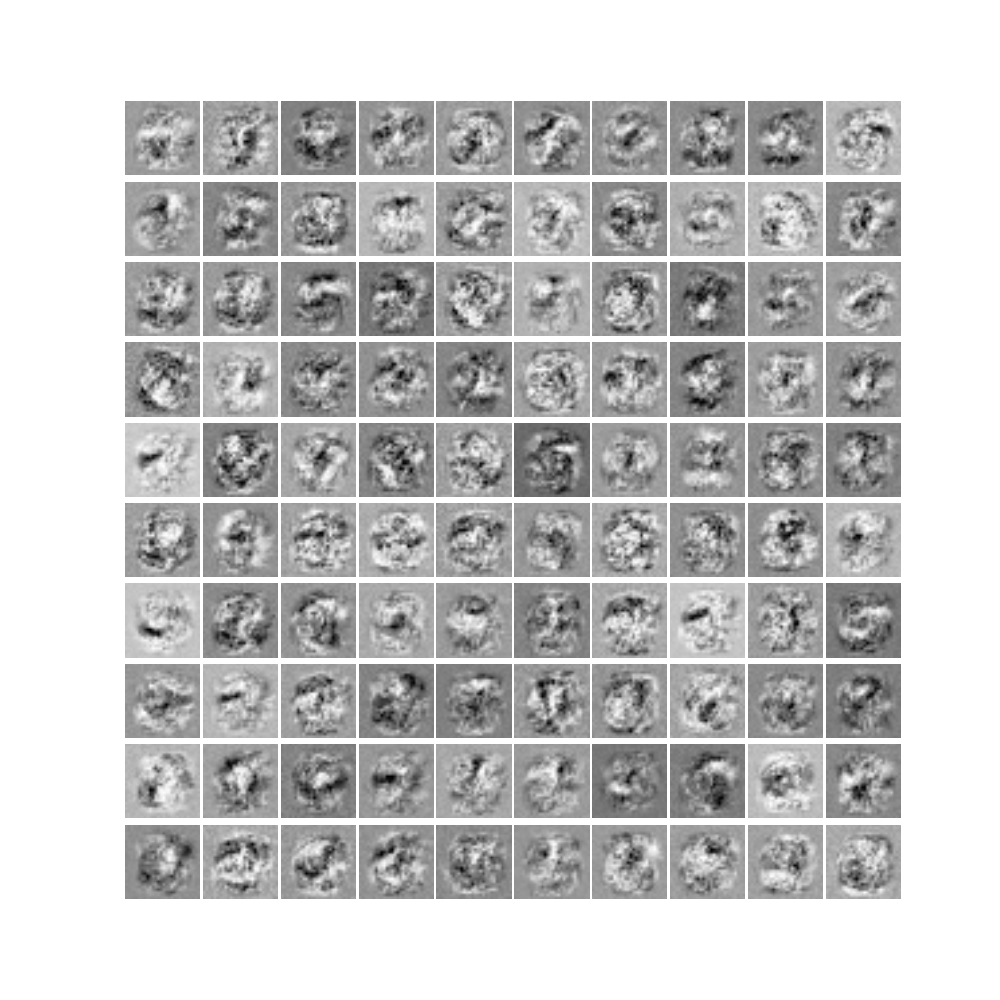
\includegraphics[width=1\textwidth]{images/problem_f_visualization} 
\end{minipage}

}
\end{figure}

\paragraph{}According to problem (d) and (e), we found $$learning\ rate = 0.01$$ $$momentum = 0$$ $$hidden\ dimension = 100$$ is the most suitable parameter for this task. Then I tried some L2 regularization coefficients and find out $$L2\ coefficient = 0.0001$$  $$epoch\ number = 180$$is the best choice.

		$$train\_loss\_cross\_entropy =  0.03, valid\_loss\_cross\_entropy = 0.27,  test\_loss\_cross\_entropy = 0.33$$
		$$train\_loss\_\%incorrect = 0.0, valid\_loss\_\%incorrect = 0.08, test\_loss\_\%incorrect = 0.09$$

\subsection{(g)}
\paragraph{} After cross validation, we find out the following parameters.
$$learning\ rate = 0.01$$ $$momentum = 0$$
$$L2\ coefficient = 0.01$$  $$epoch\ number = 140$$

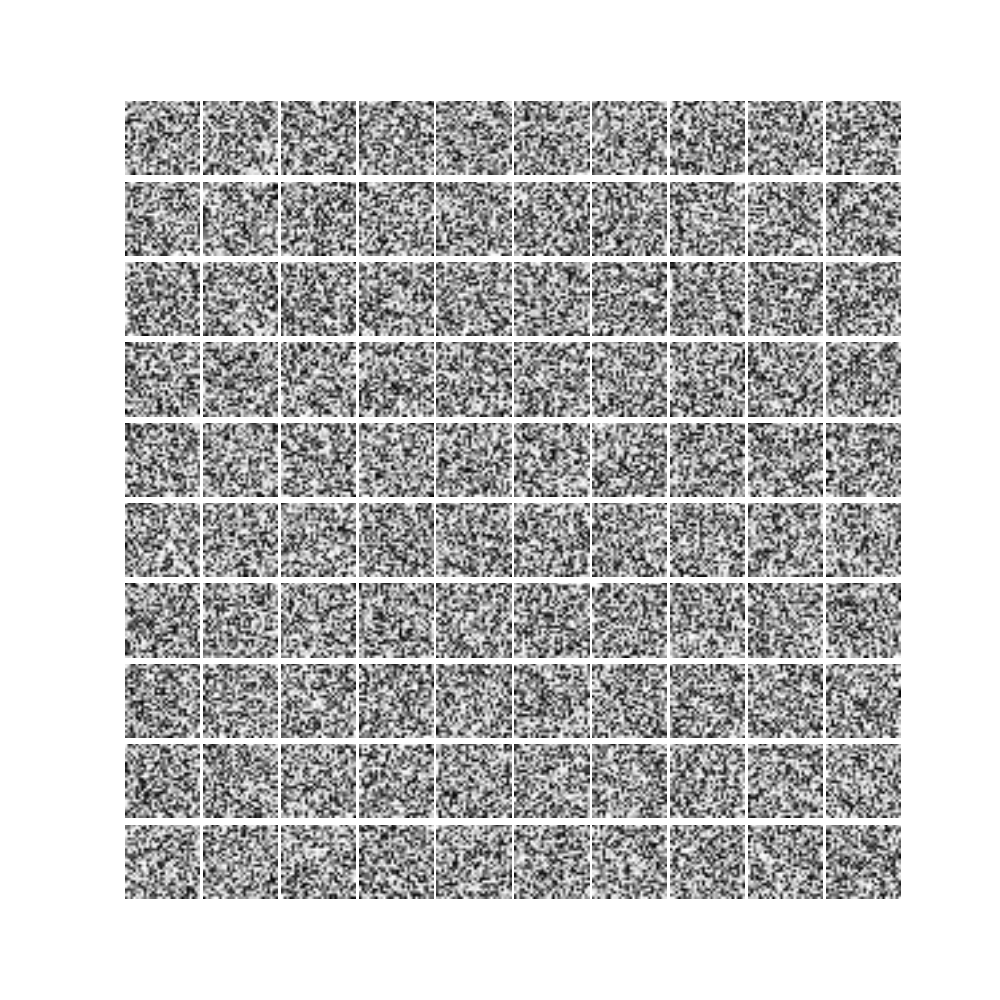
\includegraphics[width=0.5\linewidth]{images/problem_g_visualization}
\paragraph{} I cannot find out any structure in the visualization of first layer. It's much worse than the ones that I obtained when training a single-layer network.
\paragraph{} The 1-layer network outperform a 2-layer model in term of generalization capabilities.

		$$train\_loss\_cross\_entropy =  0.32, valid\_loss\_cross\_entropy = 0.50,  test\_loss\_cross\_entropy = 0.55$$
		$$train\_loss\_\%incorrect = 0.10, valid\_loss\_\%incorrect = 0.15, test\_loss\_\%incorrect = 0.17$$

\subsection{(h)}
\paragraph{}Batch normalization helps in terms of speed and accuracy. Before I use batch normalization, I need to set $learning\_rate = 0.01$ and train 140 epochs. After I use batch normalization, I can set $learning\_rate = 0.1$ and only train 7 epochs and get better result. 
		$$train\_loss\_cross\_entropy =  0.12, valid\_loss\_cross\_entropy = 0.36,  test\_loss\_cross\_entropy = 0.53$$
		$$train\_loss\_\%incorrect = 0.04, valid\_loss\_\%incorrect = 0.12, test\_loss\_\%incorrect = 0.14$$



\subsection{(i)}
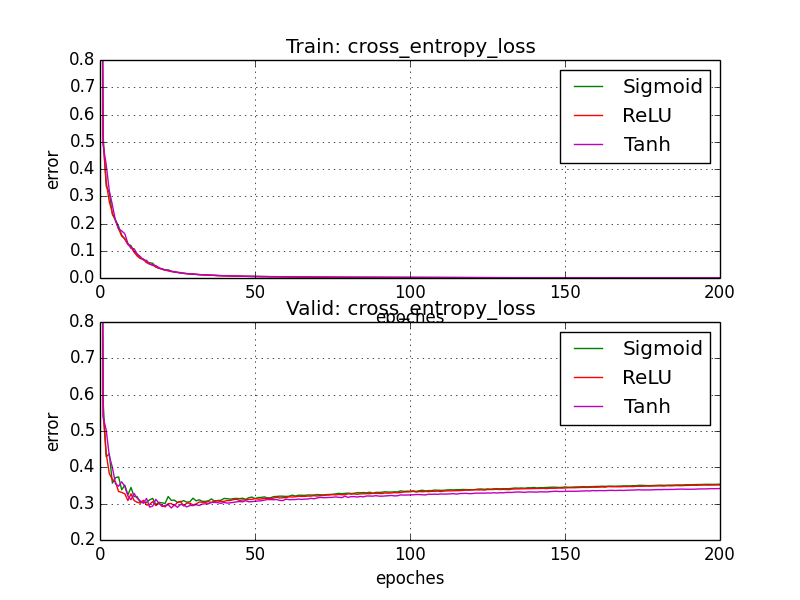
\includegraphics[width=0.5\linewidth]{images/problem_i}
\paragraph{}
I use three different activation function to train the model. The performances of Sigmoid and ReLu are almost the same, and Tanh performs slightly better than them.




\end{document}

\grid